% fig02_ladder — the 7-stage propulsion ladder with the proven/UNPROVEN wall.
% Standalone pgfplots/TikZ; compiled to figures/fig02_ladder.pdf by `make figures`.
% Comparison (stage tier across the ladder) => chart (commons comparison-chart rule).
\documentclass[tikz,border=4pt]{standalone}
\usepackage{tikz}
\usetikzlibrary{positioning,arrows.meta,fit,backgrounds}
\usepackage{xcolor}
\begin{document}
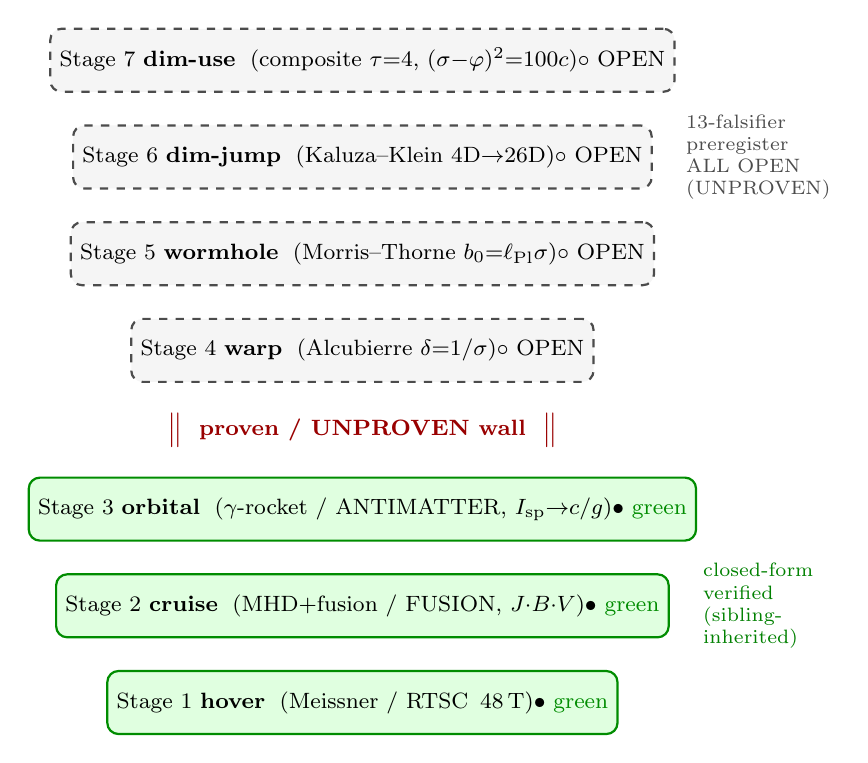
\begin{tikzpicture}[
  node distance=4mm,
  proven/.style={draw,thick,rounded corners,minimum width=58mm,minimum height=8mm,
                 fill=green!12,draw=green!55!black,align=left,font=\footnotesize},
  open/.style={draw,thick,dashed,rounded corners,minimum width=58mm,minimum height=8mm,
               fill=gray!8,draw=gray!60!black,align=left,font=\footnotesize},
]
% upper four (UNPROVEN) at top, lower three (proven) at bottom
\node[open]   (s7) {Stage 7 \textbf{dim-use} \;(composite $\tau{=}4$, $(\sigma{-}\varphi)^2{=}100c$)\hfill$\circ$ OPEN};
\node[open,below=of s7] (s6) {Stage 6 \textbf{dim-jump} \;(Kaluza--Klein 4D$\to$26D)\hfill$\circ$ OPEN};
\node[open,below=of s6] (s5) {Stage 5 \textbf{wormhole} \;(Morris--Thorne $b_0{=}\ell_{\mathrm{Pl}}\sigma$)\hfill$\circ$ OPEN};
\node[open,below=of s5] (s4) {Stage 4 \textbf{warp} \;(Alcubierre $\delta{=}1/\sigma$)\hfill$\circ$ OPEN};
% the wall
\node[below=2.5mm of s4, font=\footnotesize\bfseries, text=red!60!black] (wall)
  {$\big\Vert$\; proven / UNPROVEN wall \;$\big\Vert$};
\node[proven,below=2.5mm of wall] (s3) {Stage 3 \textbf{orbital} \;($\gamma$-rocket / ANTIMATTER, $I_{\mathrm{sp}}{\to}c/g$)\hfill$\bullet$ \textcolor{green!55!black}{green}};
\node[proven,below=of s3] (s2) {Stage 2 \textbf{cruise} \;(MHD$+$fusion / FUSION, $J{\cdot}B{\cdot}V$)\hfill$\bullet$ \textcolor{green!55!black}{green}};
\node[proven,below=of s2] (s1) {Stage 1 \textbf{hover} \;(Meissner / RTSC \,48\,T)\hfill$\bullet$ \textcolor{green!55!black}{green}};
% caption-ish side labels
\node[right=3mm of s6, font=\scriptsize, text=gray!60!black, align=left] {13-falsifier\\preregister\\ALL OPEN\\(UNPROVEN)};
\node[right=3mm of s2, font=\scriptsize, text=green!50!black, align=left] {closed-form\\verified\\(sibling-\\inherited)};
\end{tikzpicture}
\end{document}
